% Options for packages loaded elsewhere
\PassOptionsToPackage{unicode}{hyperref}
\PassOptionsToPackage{hyphens}{url}
\PassOptionsToPackage{dvipsnames,svgnames,x11names}{xcolor}
%
\documentclass[
]{article}

\usepackage{amsmath,amssymb}
\usepackage{iftex}
\ifPDFTeX
  \usepackage[T1]{fontenc}
  \usepackage[utf8]{inputenc}
  \usepackage{textcomp} % provide euro and other symbols
\else % if luatex or xetex
  \usepackage{unicode-math}
  \defaultfontfeatures{Scale=MatchLowercase}
  \defaultfontfeatures[\rmfamily]{Ligatures=TeX,Scale=1}
\fi
\usepackage{lmodern}
\ifPDFTeX\else  
    % xetex/luatex font selection
  \setmainfont[]{Latin Modern Roman}
  \setmathfont[]{Latin Modern Math}
\fi
% Use upquote if available, for straight quotes in verbatim environments
\IfFileExists{upquote.sty}{\usepackage{upquote}}{}
\IfFileExists{microtype.sty}{% use microtype if available
  \usepackage[]{microtype}
  \UseMicrotypeSet[protrusion]{basicmath} % disable protrusion for tt fonts
}{}
\makeatletter
\@ifundefined{KOMAClassName}{% if non-KOMA class
  \IfFileExists{parskip.sty}{%
    \usepackage{parskip}
  }{% else
    \setlength{\parindent}{0pt}
    \setlength{\parskip}{6pt plus 2pt minus 1pt}}
}{% if KOMA class
  \KOMAoptions{parskip=half}}
\makeatother
\usepackage{xcolor}
\setlength{\emergencystretch}{3em} % prevent overfull lines
\setcounter{secnumdepth}{5}
% Make \paragraph and \subparagraph free-standing
\ifx\paragraph\undefined\else
  \let\oldparagraph\paragraph
  \renewcommand{\paragraph}[1]{\oldparagraph{#1}\mbox{}}
\fi
\ifx\subparagraph\undefined\else
  \let\oldsubparagraph\subparagraph
  \renewcommand{\subparagraph}[1]{\oldsubparagraph{#1}\mbox{}}
\fi


\providecommand{\tightlist}{%
  \setlength{\itemsep}{0pt}\setlength{\parskip}{0pt}}\usepackage{longtable,booktabs,array}
\usepackage{calc} % for calculating minipage widths
% Correct order of tables after \paragraph or \subparagraph
\usepackage{etoolbox}
\makeatletter
\patchcmd\longtable{\par}{\if@noskipsec\mbox{}\fi\par}{}{}
\makeatother
% Allow footnotes in longtable head/foot
\IfFileExists{footnotehyper.sty}{\usepackage{footnotehyper}}{\usepackage{footnote}}
\makesavenoteenv{longtable}
\usepackage{graphicx}
\makeatletter
\def\maxwidth{\ifdim\Gin@nat@width>\linewidth\linewidth\else\Gin@nat@width\fi}
\def\maxheight{\ifdim\Gin@nat@height>\textheight\textheight\else\Gin@nat@height\fi}
\makeatother
% Scale images if necessary, so that they will not overflow the page
% margins by default, and it is still possible to overwrite the defaults
% using explicit options in \includegraphics[width, height, ...]{}
\setkeys{Gin}{width=\maxwidth,height=\maxheight,keepaspectratio}
% Set default figure placement to htbp
\makeatletter
\def\fps@figure{htbp}
\makeatother
% definitions for citeproc citations
\NewDocumentCommand\citeproctext{}{}
\NewDocumentCommand\citeproc{mm}{%
  \begingroup\def\citeproctext{#2}\cite{#1}\endgroup}
\makeatletter
 % allow citations to break across lines
 \let\@cite@ofmt\@firstofone
 % avoid brackets around text for \cite:
 \def\@biblabel#1{}
 \def\@cite#1#2{{#1\if@tempswa , #2\fi}}
\makeatother
\newlength{\cslhangindent}
\setlength{\cslhangindent}{1.5em}
\newlength{\csllabelwidth}
\setlength{\csllabelwidth}{3em}
\newenvironment{CSLReferences}[2] % #1 hanging-indent, #2 entry-spacing
 {\begin{list}{}{%
  \setlength{\itemindent}{0pt}
  \setlength{\leftmargin}{0pt}
  \setlength{\parsep}{0pt}
  % turn on hanging indent if param 1 is 1
  \ifodd #1
   \setlength{\leftmargin}{\cslhangindent}
   \setlength{\itemindent}{-1\cslhangindent}
  \fi
  % set entry spacing
  \setlength{\itemsep}{#2\baselineskip}}}
 {\end{list}}
\usepackage{calc}
\newcommand{\CSLBlock}[1]{\hfill\break\parbox[t]{\linewidth}{\strut\ignorespaces#1\strut}}
\newcommand{\CSLLeftMargin}[1]{\parbox[t]{\csllabelwidth}{\strut#1\strut}}
\newcommand{\CSLRightInline}[1]{\parbox[t]{\linewidth - \csllabelwidth}{\strut#1\strut}}
\newcommand{\CSLIndent}[1]{\hspace{\cslhangindent}#1}

\usepackage{arxiv}
\usepackage{orcidlink}
\usepackage{amsmath}
\usepackage[T1]{fontenc}
\makeatletter
\@ifpackageloaded{caption}{}{\usepackage{caption}}
\AtBeginDocument{%
\ifdefined\contentsname
  \renewcommand*\contentsname{Table of contents}
\else
  \newcommand\contentsname{Table of contents}
\fi
\ifdefined\listfigurename
  \renewcommand*\listfigurename{List of Figures}
\else
  \newcommand\listfigurename{List of Figures}
\fi
\ifdefined\listtablename
  \renewcommand*\listtablename{List of Tables}
\else
  \newcommand\listtablename{List of Tables}
\fi
\ifdefined\figurename
  \renewcommand*\figurename{Figure}
\else
  \newcommand\figurename{Figure}
\fi
\ifdefined\tablename
  \renewcommand*\tablename{Table}
\else
  \newcommand\tablename{Table}
\fi
}
\@ifpackageloaded{float}{}{\usepackage{float}}
\floatstyle{ruled}
\@ifundefined{c@chapter}{\newfloat{codelisting}{h}{lop}}{\newfloat{codelisting}{h}{lop}[chapter]}
\floatname{codelisting}{Listing}
\newcommand*\listoflistings{\listof{codelisting}{List of Listings}}
\makeatother
\makeatletter
\makeatother
\makeatletter
\@ifpackageloaded{caption}{}{\usepackage{caption}}
\@ifpackageloaded{subcaption}{}{\usepackage{subcaption}}
\makeatother
\ifLuaTeX
  \usepackage{selnolig}  % disable illegal ligatures
\fi
\usepackage{bookmark}

\IfFileExists{xurl.sty}{\usepackage{xurl}}{} % add URL line breaks if available
\urlstyle{same} % disable monospaced font for URLs
\hypersetup{
  pdftitle={Comparison of Catalogs},
  colorlinks=true,
  linkcolor={blue},
  filecolor={Maroon},
  citecolor={Blue},
  urlcolor={Blue},
  pdfcreator={LaTeX via pandoc}}

\newcommand{\runninghead}{A Preprint }
\title{Comparison of Catalogs}
\def\asep{\\\\\\ } % default: all authors on same column
\author{}
\date{}
\begin{document}
\maketitle

\renewcommand*\contentsname{Table of contents}
{
\hypersetup{linkcolor=}
\setcounter{tocdepth}{3}
\tableofcontents
}
\section{The data}\label{the-data}

In this script we will compare 2 catalogs, HECATE (Kovlakas et al.
(2021)) and LVG (Karachentsev and Kaisina (2013))

\begin{itemize}
\tightlist
\item
  The data have been joined based on their position in the sky (Ra,
  Dec).

  \begin{itemize}
  \tightlist
  \item
    We assume that every galaxy within 2 arc seconds of the initial
    coordinates is the same galaxy.
  \end{itemize}
\item
  We use TOPCAT to create two joins, an inner and an outer join
\item
  We will use the inner join for 1-1 comparisons
\item
  If we see that the data are similar we can use the outer join
\item
  For the comparison we keep the parameters names exactly they are given
  in the catalogs
\end{itemize}

The dataset we are going to use for the comparison (inner join) consists
of 3934 galaxies and 172 columns with their physical characteristics.

\section{Catalog Completeness}\label{catalog-completeness}

Checking for completeness in galaxy catalogs is essential to ensure that
the data accurately represents the true population of galaxies, for
\(z \approx 0\). Incomplete catalogs can lead to biased results in
statistical studies, such as the distribution of galaxy luminosity,
mass, or star formation rates. Additionally, missing galaxies,
especially those at faint magnitudes or large distances, can distort
cosmological measurements and hinder our understanding of galaxy
formation and evolution.

Completeness checks are crucial for addressing selection biases,
identify gaps in the data and guide follow-up observations, ensuring
that the catalog provides a reliable sample for scientific analysis.
Without these checks, conclusions drawn from the data may be inaccurate
or incomplete.

\subsection{Completeness of the LVG
Catalog}\label{completeness-of-the-lvg-catalog}

The local volume selection has been made by taking into account galaxies
with:

\begin{enumerate}
\def\labelenumi{\arabic{enumi}.}
\tightlist
\item
  Radial velocities of
\end{enumerate}

\begin{equation}\phantomsection\label{eq-lvg-vel}{
     V_{LG}<600 \text{ km}\cdot\text{m}^{-1}
}\end{equation}

\begin{enumerate}
\def\labelenumi{\arabic{enumi}.}
\tightlist
\item
  Distances of
\end{enumerate}

\begin{equation}\phantomsection\label{eq-lvg-dis}{
       D<11\ \text{Mpc}
}\end{equation}

A simultaneous fulfillment of both conditions (1) and (2) is not
required.

\subsubsection{Difficulties in calculating the
Completeness}\label{difficulties-in-calculating-the-completeness}

As explained in (Karachentsev, Makarov, and Kaisina (2013)), it is
difficult to calculate the completeness of the catalog.

\begin{enumerate}
\def\labelenumi{\arabic{enumi}.}
\tightlist
\item
  Completeness within a 10 Mpc radius is difficult to assess due to: -
  Variability in galaxy properties (luminosity, size, surface
  brightness, gas content) - Errors in distance measurements
  (Tully--Fisher method errors of \textasciitilde20--25\%), especially
  at the 10 Mpc boundary.

  \begin{itemize}
  \tightlist
  \item
    Accurate distances are mainly known within \textasciitilde5 Mpc.
  \item
    Non-Hubble motions (\textasciitilde300 km/s)\footnote{\emph{Non-Hubble
      motion refers to the component of a galaxy's velocity that
      deviates from the uniform expansion of the universe, described by
      the equation} \(V= H_0 d + v_p\),where \(V\) is the total
      velocity, \(H_0 d\) represents the Hubble flow, and
      \(v_p\)\hspace{0pt} is the peculiar velocity. {``Essay''} (n.d.)}
    may make up half of the adopted velocity constraint
    (Equation~\ref{eq-lvg-vel})

    \begin{itemize}
    \tightlist
    \item
      Solution for our usage: only keep the galaxies inside a radius of
      \(D=11 Mpc\)
    \end{itemize}
  \item
    HI sources in surveys with low angular resolution: ``The presence
    around our Galaxy of hundreds of high-velocity clouds with low
    line-of-sight velocities and small W50 widths also provokes the
    inclusion of false ``nearby'' dwarf galaxies in the
    LV''(Karachentsev, Makarov, and Kaisina (2013))
  \end{itemize}
\end{enumerate}

\begin{enumerate}
\def\labelenumi{\arabic{enumi}.}
\setcounter{enumi}{1}
\tightlist
\item
  Astro-Spam and Survey Errors:

  \begin{itemize}
  \tightlist
  \item
    Automatic surveys produce false detections (e.g., stars
    misclassified as galaxies, high-velocity clouds mistaken for
    dwarfs).
  \end{itemize}
\item
  Conditional Completeness Estimate: - Galaxies brighter than
  \(M_B^c = -11^m\) or with linear diameters larger than
  \(A_{26} = 1.0\) kpc show (40--60)\% completeness.

  \begin{itemize}
  \tightlist
  \item
    ``among the members of the Local Group (D \textless{} 1 Mpc), only
    half of the galaxies have absolute magnitudes brighter than
    \(−11^m\). Consequently, more than half of the ultra-faint dwarf
    companions around normal galaxies, like the Sombrero galaxy (D = 9.3
    Mpc), still remain outside our field of view.''
  \end{itemize}
\item
  Undetected Ultra-Faint Dwarfs:

  \begin{itemize}
  \tightlist
  \item
    Many faint dwarf galaxies remain undetected beyond the Local Group.
    Estimated population of undetected dwarfs could be as large as
    \(10^3–10^4\) within the LV.
  \end{itemize}
\item
  Surface Brightness Distribution:

  \begin{itemize}
  \tightlist
  \item
    Surface brightness remains consistent across distances, except for
    ultra-faint dwarfs (\(SB <31 \text{mag}\cdot\text{arcsec}^{-2}\)).
  \item
    Faintest dwarf galaxies are detectable only nearby due to their
    resolution into individual stars.
  \end{itemize}
\item
  Luminosity-Size Relationship:

  \begin{itemize}
  \tightlist
  \item
    Observations align with cosmological models predicting \(L\sim A^3\)
    (Navarro, Frenk, and White (1996)), though deviations occur for
    extremely low surface brightness galaxies.
  \item
    ``The deviation from it at the extremely low surface brightness end
    is due to a systematic overestimation of dwarf galaxy sizes, the
    brightness profiles of which lie entirely below the Holmberg
    isophote.''
  \end{itemize}
\end{enumerate}

\subsection{Completeness of HECATE}\label{completeness-of-hecate}

The completeness of HECATE is difficult to assess due to: - Unknown
selection function of HyperLEDA and selection effects from other
cross-correlated catalogs. - Estimation based on comparing B-band
luminosity distribution with the galaxy luminosity function (LF).

\begin{itemize}
\item
  HECATE is:

  \begin{itemize}
  \item
    Complete down to \(L_B\sim 10^{9.5} L_{B,\odot}\) for distances less
    than 33 Mpc.
  \item
    Complete down to \(L_B\sim 10^{10} L_{B,\odot}\) for distances
    between 67 Mpc and 100 Mpc.
  \item
    Incomplete at distances greater than 167 Mpc, even for the brightest
    galaxies.
  \end{itemize}
\item
  Completeness estimates based on B-band luminosity density:

  \begin{itemize}
  \item
    \textgreater75\% complete for distances less than 100 Mpc.
    \(\sim 50\%\) complete at distances of \(\sim170\) Mpc.
  \item
    Completeness exceeds 100\% within 30 Mpc due to the overdensity of
    galaxies around the Milky Way.
  \end{itemize}
\item
  Completeness in terms of stellar mass (M*):

  \begin{itemize}
  \item
    Similar to B-band completeness when measured with \(K_s\)-band
    luminosity as a tracer for stellar mass.
  \item
    Overdensity at small distances and cut-off at large distances are
    observed.
  \end{itemize}
\item
  Completeness in terms of star formation rate (SFR):

  \begin{itemize}
  \item
    \textasciitilde50\% complete between 30 and 150 Mpc.
  \item
    Lower SFR completeness due to limitations in WISE-based SFR
    estimates, which lack full sky coverage.
  \item
    Despite IRAS's limited depth, it provides \textgreater50\% coverage
    for star-forming galaxies in the local neighborhood.
  \item
    HECATE's nonuniform SFR and stellar mass coverage, affecting the
    reliability of stellar population parameters.
  \end{itemize}
\end{itemize}

In this section we will check the completeness

\begin{longtable}[]{@{}lr@{}}
\toprule\noalign{}
Table & Number of galaxies \\
\midrule\noalign{}
\endhead
\bottomrule\noalign{}
\endlastfoot
Inner join & 3934 \\
Outer join & 3934 \\
LVG & 1321 \\
HECATE & 2901 \\
Unique galaxies in LVG & 1033 \\
Unique Galaxies in Hecate & 2613 \\
\end{longtable}

\subsection{Completeness of the Inner
join}\label{completeness-of-the-inner-join}

\[
\text{Completeness (X)}=\frac{\text{(Galaxies in Inner Join)}}{\text{(Galaxies in X)}}×100\%
\]

Completeness (HECATE)= 136 \%

Completeness (LVG)= 298 \%

\subsection{Completeness in Outer
join}\label{completeness-in-outer-join}

\[
\text{Completeness (X)}=\frac{\text{(Galaxies in Outer Join form X)}}{\text{(Galaxies in X)}}×100\%
\]

Completeness (HECATE)= 90 \%

Completeness (LVG)= 78 \%

Combined Completeness
=\(\frac{\text{Total galaxies in Outer}}{\text{Unique galaxies in HECATE + LVG}}\)=
108 \%

\subsection{Completeness of the Data}\label{completeness-of-the-data}

\begin{figure}

\begin{minipage}{0.50\linewidth}

\centering{

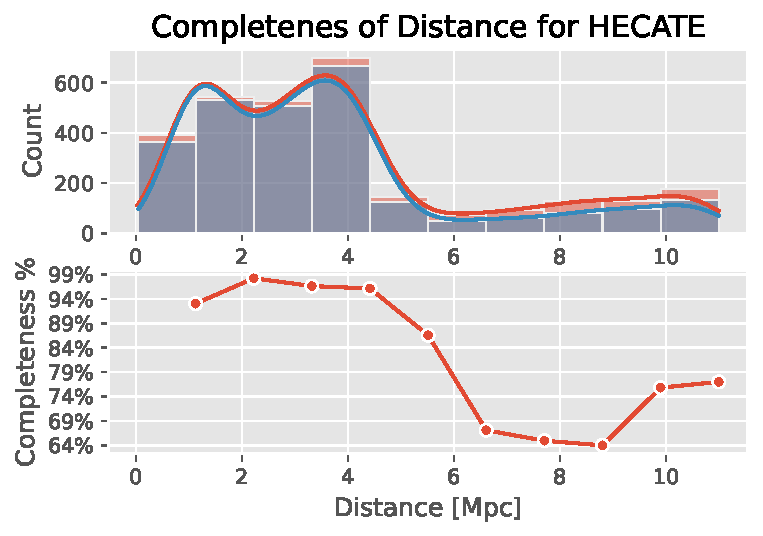
\includegraphics{compare_files/figure-pdf/fig-dis-comp-output-1.pdf}

}

\subcaption{\label{fig-dis-comp-1}HECATE}

\end{minipage}%
%
\begin{minipage}{0.50\linewidth}

\centering{

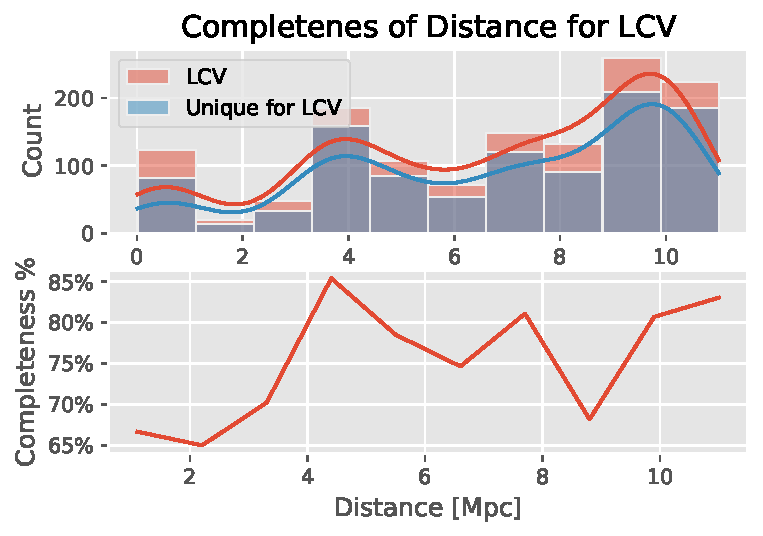
\includegraphics{compare_files/figure-pdf/fig-dis-comp-output-2.pdf}

}

\subcaption{\label{fig-dis-comp-2}LVG}

\end{minipage}%

\caption{\label{fig-dis-comp}Histograms showing the Distance
Completeness of the Catalogs}

\end{figure}%

\begin{figure}

\begin{minipage}{0.50\linewidth}

\centering{

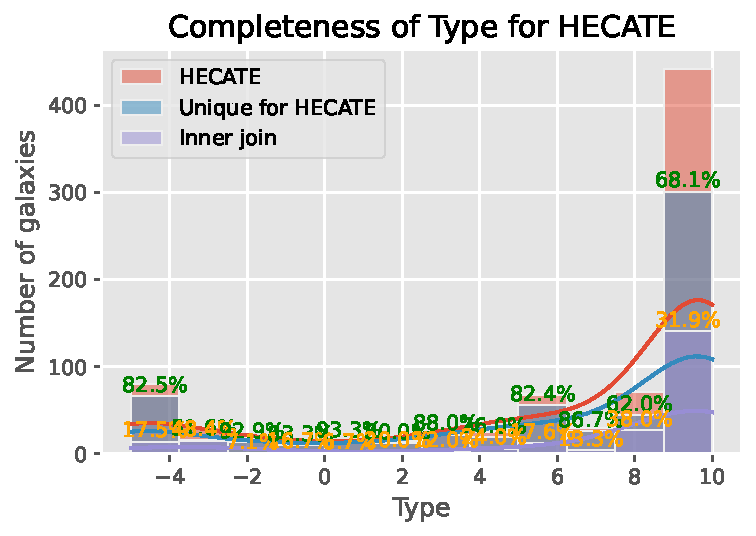
\includegraphics{compare_files/figure-pdf/fig-type-comp-output-1.pdf}

}

\subcaption{\label{fig-type-comp-1}HECATE}

\end{minipage}%
%
\begin{minipage}{0.50\linewidth}

\centering{

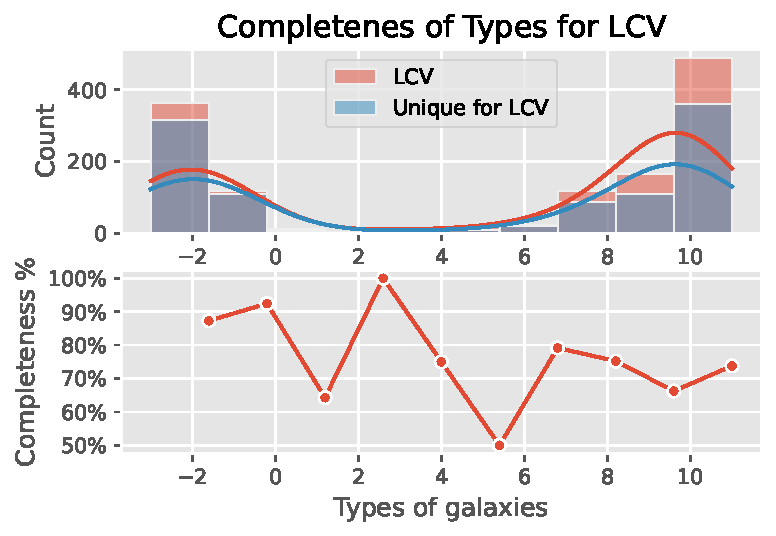
\includegraphics{compare_files/figure-pdf/fig-type-comp-output-2.pdf}

}

\subcaption{\label{fig-type-comp-2}LVG}

\end{minipage}%

\caption{\label{fig-type-comp}Histograms showing the Type Completeness
of the Catalogs}

\end{figure}%

\section{How are we going to compare the
data?}\label{how-are-we-going-to-compare-the-data}

For the comparison of our data we will mainly use two methods: linear
regression and comparison of the distributions.

For the linear regression out main tools are scatter plots and \(R^2\)

\begin{enumerate}
\def\labelenumi{\arabic{enumi}.}
\item
  \(R^2\): Measures the proportion of variance explained by the linear
  model.
\item
  Slope of the Fitted Line: Should be close to 1 for a 1-1 correlation.
\item
  Pearson Correlation \(\rho\): Measures the strength and direction of
  the linear relationship between two variables, ranging from -1 to 1.
  \footnote{In simple linear regression, \(R^2\) is the square of the
    Pearson correlation coefficient \(\rho\).}
\end{enumerate}

\begin{enumerate}
\def\labelenumi{\arabic{enumi}.}
\setcounter{enumi}{3}
\item
  Plots: Plots are essential for visually assessing the relationship
  between two datasets, identifying correlations, trends, and outliers,
  and evaluating the fit of linear models. Beside scatter plots and
  histograms, another useful plot is the Correlation Heatmap.

  \begin{quote}
  Correlation Heatmaps: A correlation heatmap is a graphical tool that
  displays the correlation between multiple variables as a color-coded
  matrix. It's like a color chart that shows us how closely related
  different variables are. In a correlation heatmap, each variable is
  represented by a row and a column, and the cells show the correlation
  between them. The color of each cell represents the strength and
  direction of the correlation, with darker colors indicating stronger
  correlations.
  \end{quote}
\end{enumerate}

For the distribution comparisons we will use histograms and Kernel
Density Estimate (KDE) plots. The KDE plots visually represent the
distribution of data, providing insights into its shape, central
tendency, and spread.

Finally, we will examine the percentage change for each galaxy.

\begin{itemize}
\tightlist
\item
  Percentage change: We can calculate the percentage change of the data
  for each galaxy and then we can see if the data are similar, based on
  minimum, the maximum and the mean value of the difference.
\end{itemize}

\[\text{Percentage change} = \frac{V_{Hecate} - V_{LVG}}{V_{Hecate}}\cdot 100 \%\]

\section{Comparable data}\label{comparable-data}

\subsection{Coordinates}\label{coordinates}

\begin{longtable}[]{@{}ccc@{}}
\toprule\noalign{}
LVG & HECATE & Description \\
\midrule\noalign{}
\endhead
\bottomrule\noalign{}
\endlastfoot
Dis & D & Distance \\
\end{longtable}

\begin{figure}

\centering{

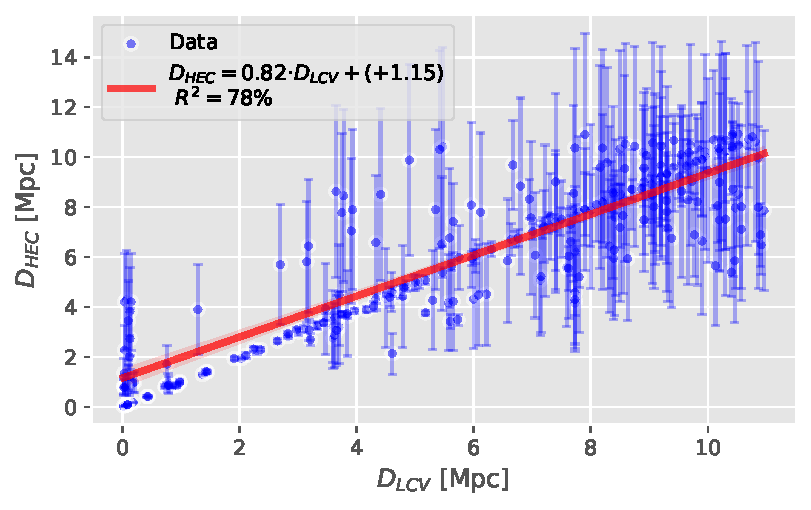
\includegraphics{compare_files/figure-pdf/fig-coord-compare-output-1.pdf}

}

\caption{\label{fig-coord-compare}Comparison of the Distances}

\end{figure}%

\begin{itemize}
\tightlist
\item
  The average error of the distance in the HECATE catalog is
  \(\overline{\delta D} = \pm 1.6\) Mpc, so the intercept is included in
  the error.
\item
  So we can assume that the Distances are the same
\end{itemize}

\subsection{Velocities}\label{velocities}

\begin{longtable}[]{@{}ccc@{}}
\toprule\noalign{}
LVG & HECATE & Description \\
\midrule\noalign{}
\endhead
\bottomrule\noalign{}
\endlastfoot
RVel (km/s) & V (km/s) & Heliocentric radial velocity \\
VLG (km/s) & & Radial velocity \\
cz (km/s) & & Heliocentric velocity \\
& V\_VIR (km/s) & Virgo-infall corrected radial velocity \\
\end{longtable}

\begin{figure}

\centering{

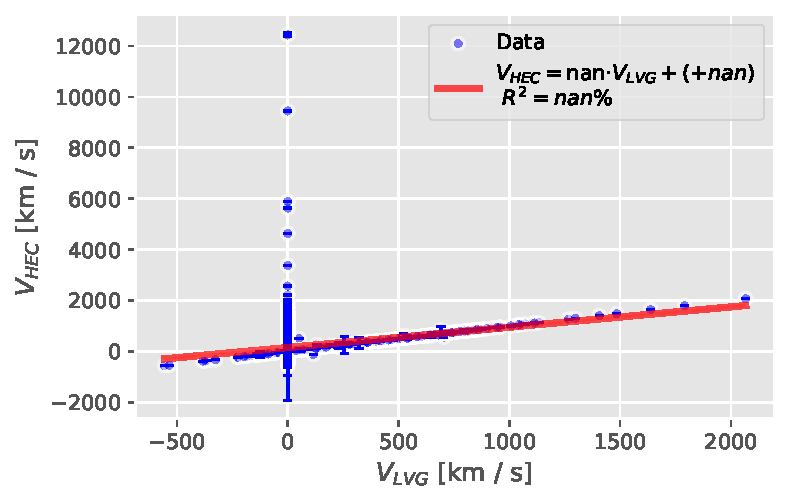
\includegraphics{compare_files/figure-pdf/fig-vel-compare-output-1.pdf}

}

\caption{\label{fig-vel-compare}Comparison of the Radial Velocities}

\end{figure}%

\begin{itemize}
\tightlist
\item
  The average error of the radial velocity in the HECATE catalog is
  \(\overline{\delta V} = \pm 12\text{km}\cdot s^{-1}\) , so the
  intercept is included in the error.
\item
  So we can assume that the radial velocities are the same
\end{itemize}

\begin{figure}

\centering{

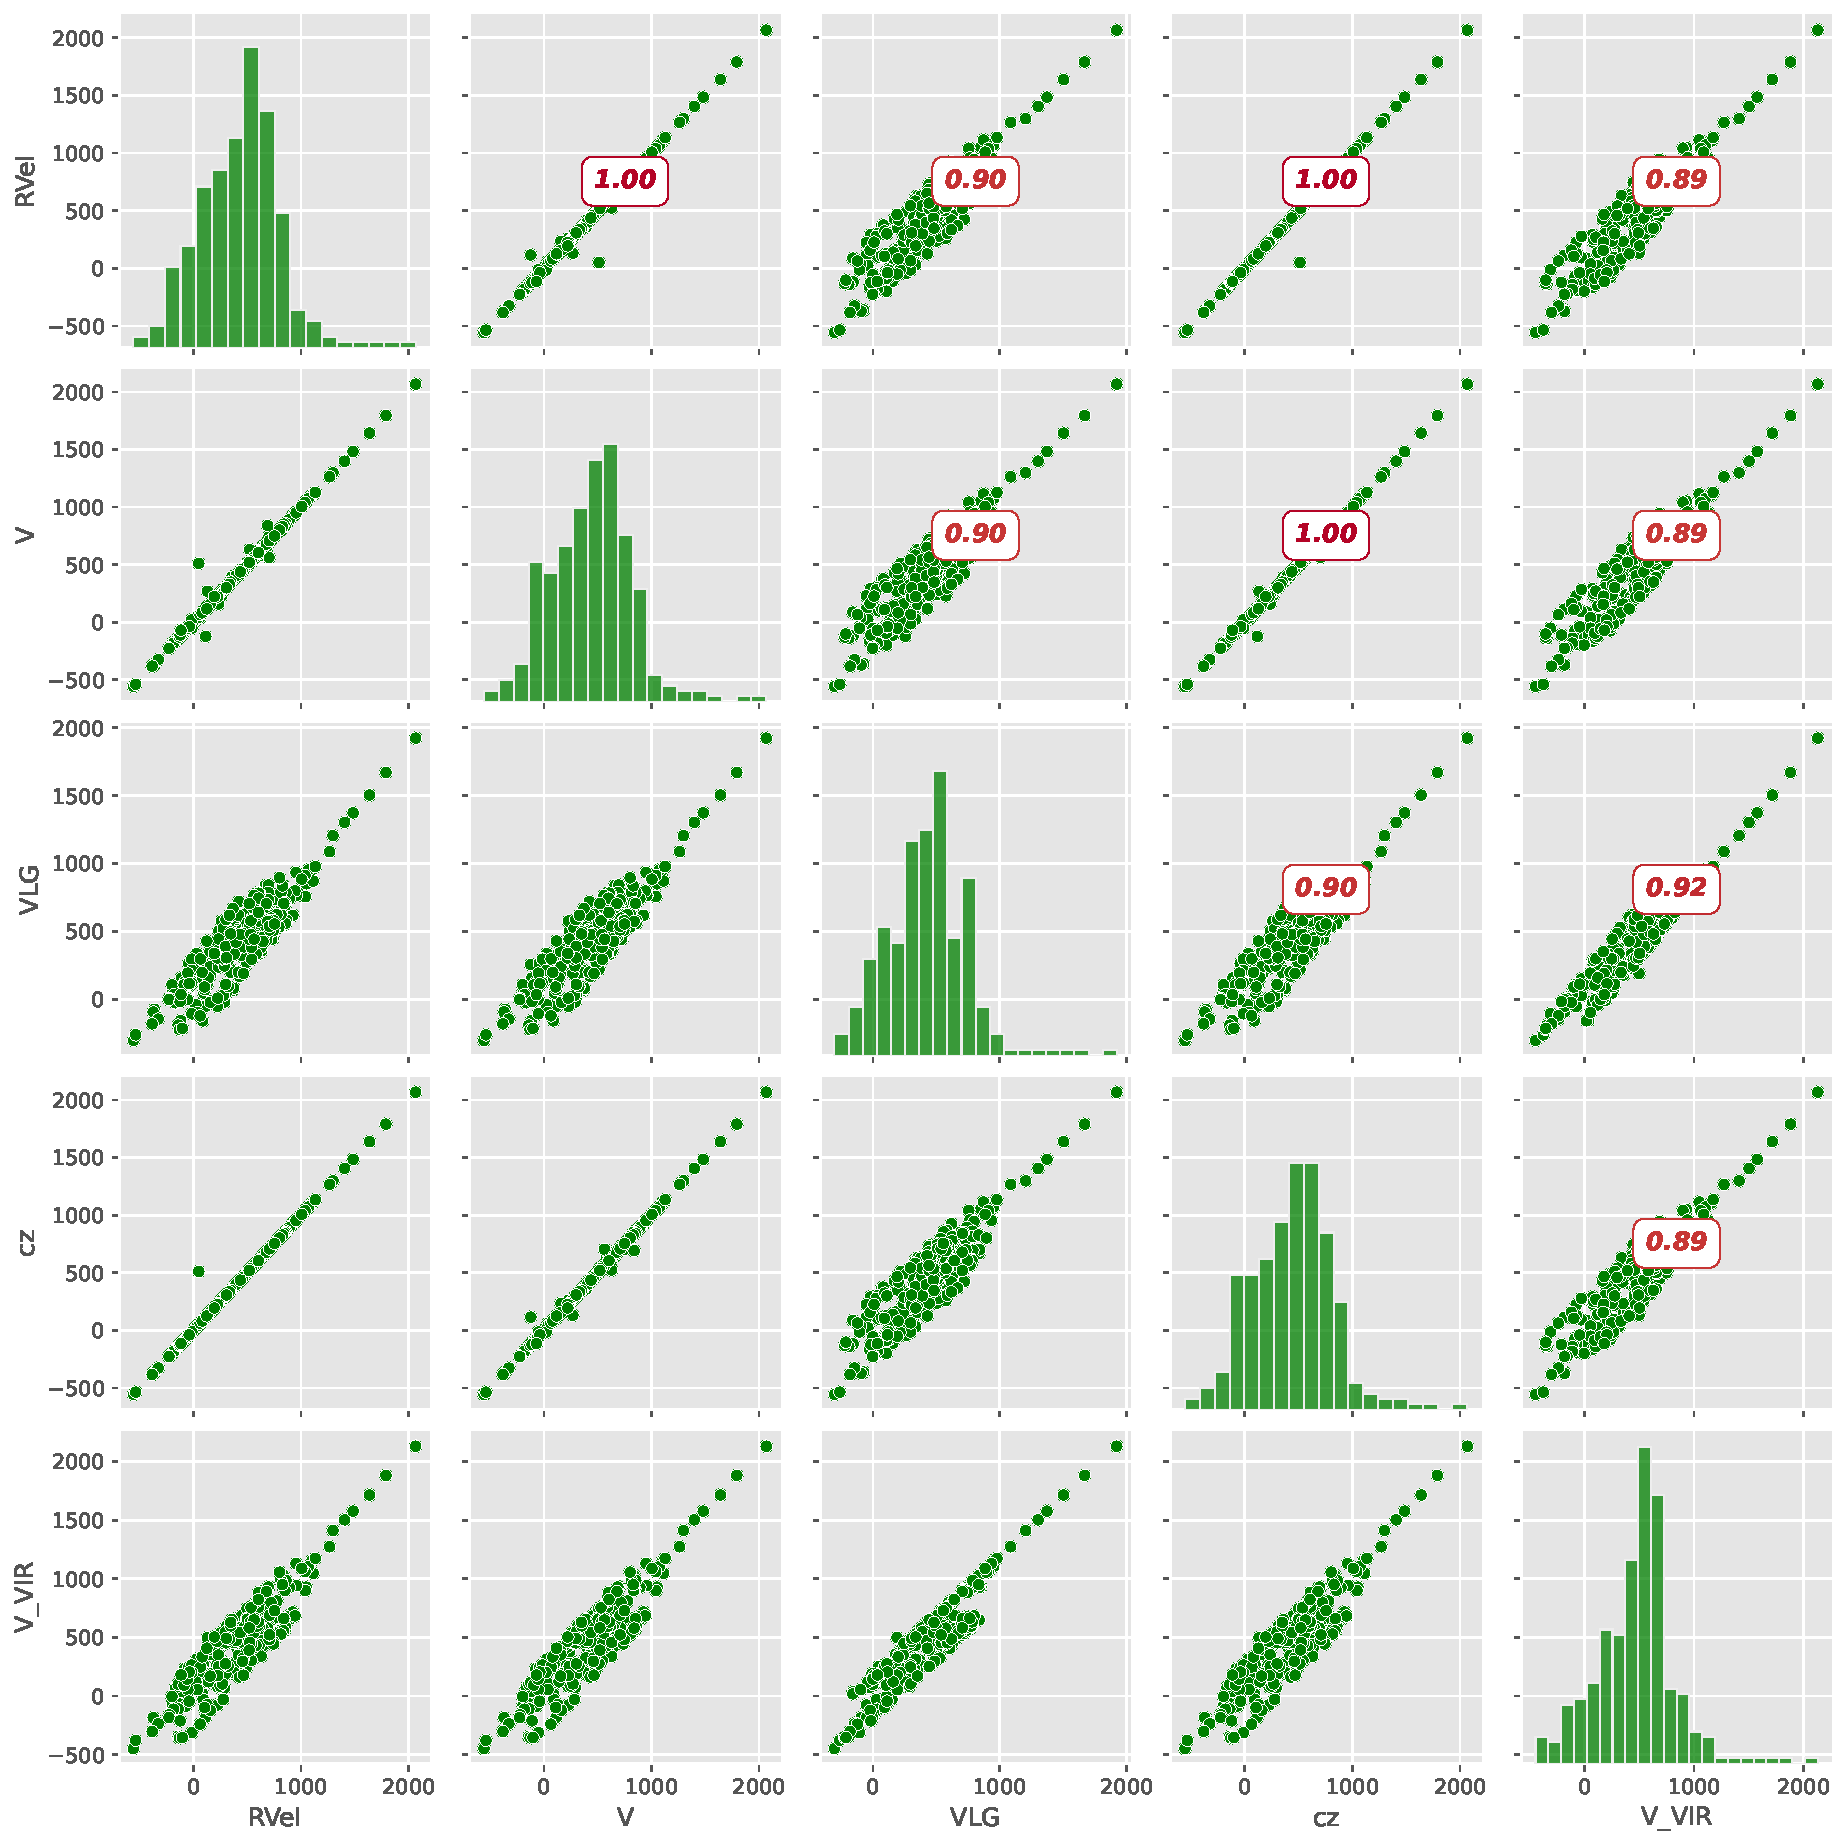
\includegraphics{compare_files/figure-pdf/fig-vel-pairplot-output-1.pdf}

}

\caption{\label{fig-vel-pairplot}The correlation Matrix of the
Velocities. The lower left triangle is composed of the scatter plots of
the various velocities, the diagonal shows their distrubution and the
upper right triangle shows the correlations of the Velocities}

\end{figure}%

{[}?{]} The strong correlation between the velocities reported by the
HECATE and LVG catalogs (Figure~\ref{fig-vel-pairplot}) can be
attributed to the fact that both measure the same intrinsic galaxy
velocities but reference them to different frames. For instance,
velocities can be corrected for the movement of the Earth (heliocentric
frame) or the for the Virgo-infall. These corrections shift the measured
velocity slightly, but the fundamental measurement remains consistent.
This explains why the velocities are highly correlated, as they
represent the same physical phenomenon but adjusted for different
reference points.

\newpage{}

\subsection{Morphology and Geometry}\label{morphology-and-geometry}

\begin{longtable}[]{@{}
  >{\centering\arraybackslash}p{(\columnwidth - 4\tabcolsep) * \real{0.3273}}
  >{\centering\arraybackslash}p{(\columnwidth - 4\tabcolsep) * \real{0.3273}}
  >{\centering\arraybackslash}p{(\columnwidth - 4\tabcolsep) * \real{0.3455}}@{}}
\toprule\noalign{}
\begin{minipage}[b]{\linewidth}\centering
LVG
\end{minipage} & \begin{minipage}[b]{\linewidth}\centering
HECATE
\end{minipage} & \begin{minipage}[b]{\linewidth}\centering
Description
\end{minipage} \\
\midrule\noalign{}
\endhead
\bottomrule\noalign{}
\endlastfoot
TType & T (with errors) & Numerical Hubble type following the de
Vaucouleurs system \\
inc & INCL & Inclination (deg) \\
a26\_1 (Major) & R1 (Semi-major axis) & angular diameter (arcmin) \\
\end{longtable}

\subsubsection{Galaxy Types}

``Morphological type of galaxy in the numerical code according to the
classification by de Vaucouleurs et al.~(1991). It should be noted that
about three quarters of objects in the LV are dwarf galaxies, which
require a more detailed morphological classification. For example, dwarf
spheroidal galaxies and normal ellipticals are usually denoted by the
same numerical code T \textless{} 0, although their physical properties
drastically differ. The classification problem arises as well for the
``transient'' type dwarf galaxies, T r, which combine the features of
spheroidal (Sph) and irregular (Ir)systems. Due to small classification
errors, such objects may ``jump'' from one end of the T scale to the
other.'' (Karachentsev, Makarov, and Kaisina (2013))

``as they correspond to types T \textless{} 1. The shortcomings of such
a simplified classification of dwarf systems have become apparent;
hence, van den Bergh (1959) proposed a more refined scheme where dwarf
galaxies were assumed to be divided by luminosity class\ldots Such an
approach allowed us to avoid unpleasant cases in which a dwarf galaxy of
intermediate type jumps over due to a misclassification from one end of
the de Vaucouleurs sequence (T \textless{} 1) to the other (T = 9,
10).'' (Karachentsev and Kaisina (2013))

\begin{figure}

\begin{minipage}{0.50\linewidth}

\centering{

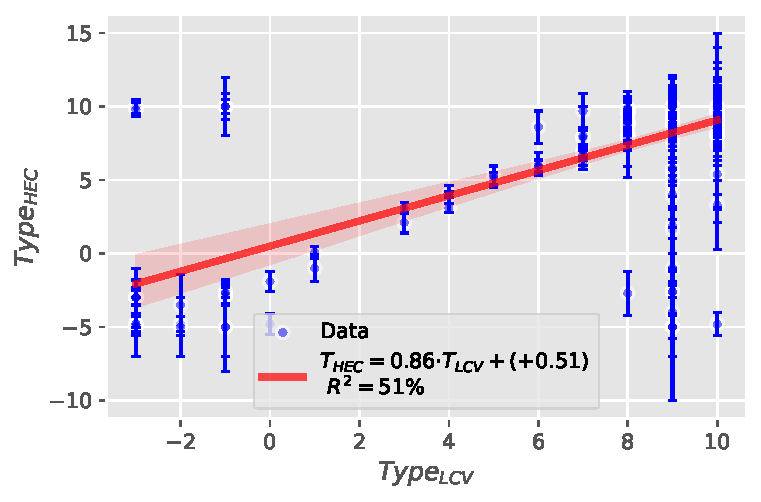
\includegraphics{compare_files/figure-pdf/fig-types-compare-output-1.pdf}

}

\subcaption{\label{fig-types-compare-1}All the galaxies, without the
correction}

\end{minipage}%
%
\begin{minipage}{0.50\linewidth}

\centering{

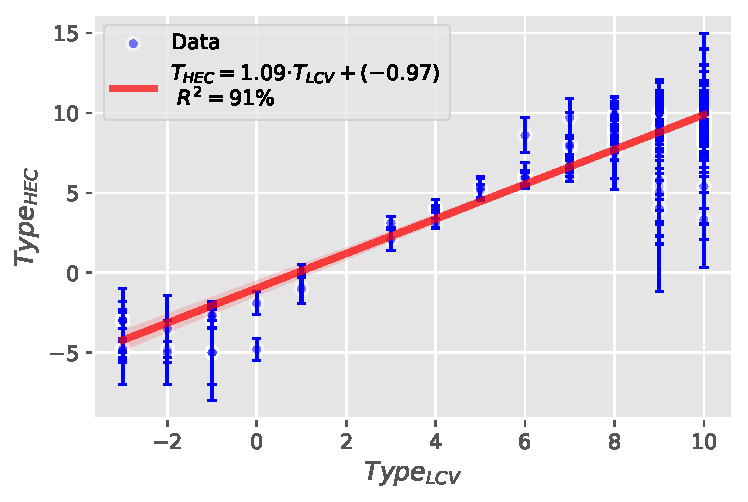
\includegraphics{compare_files/figure-pdf/fig-types-compare-output-2.pdf}

}

\subcaption{\label{fig-types-compare-2}Comparison with the correction
\(|{T_{HECATE}-T_{LVG}}|<σ_{Τ_{LVG}}\)}

\end{minipage}%

\caption{\label{fig-types-compare}Comparison of the Types of galaxies}

\end{figure}%

\begin{itemize}
\tightlist
\item
  we can assume that the galaxies from the upper left and lower right
  regions of the plot are classified differently because of this
\item
  this might explain the large errors \(\delta T\) of HECATE
\item
  why we see a difference in the distribution of
  (Figure~\ref{fig-type-comp})
\end{itemize}

We can remove the ``problematic'' galaxies by only keeping the ones
with: \[
|{T_{HECATE}-T_{LVG}}|<\sigma_{T_{LVG}} = 4.8
\]

\begin{itemize}
\tightlist
\item
  The average uncertainty of the morphological type in the HECATE
  catalog is \(\overline{\delta T} = \pm 1.4\), so the intercept is
  included in the error.
\item
  So we can assume that the Morphological Types are the same
\end{itemize}

\subsubsection{Inclination}

\begin{figure}

\begin{minipage}{0.50\linewidth}

\centering{

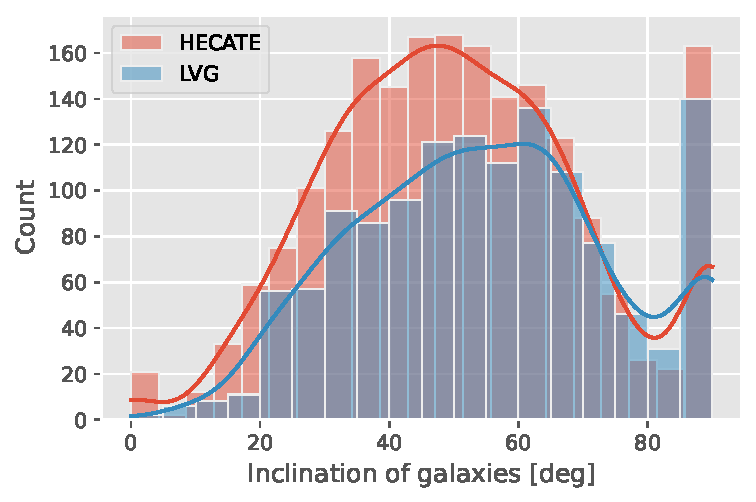
\includegraphics{compare_files/figure-pdf/fig-incl-compare-output-1.pdf}

}

\subcaption{\label{fig-incl-compare-1}Distribution of the Inclination of
the galaxies}

\end{minipage}%
%
\begin{minipage}{0.50\linewidth}

\centering{

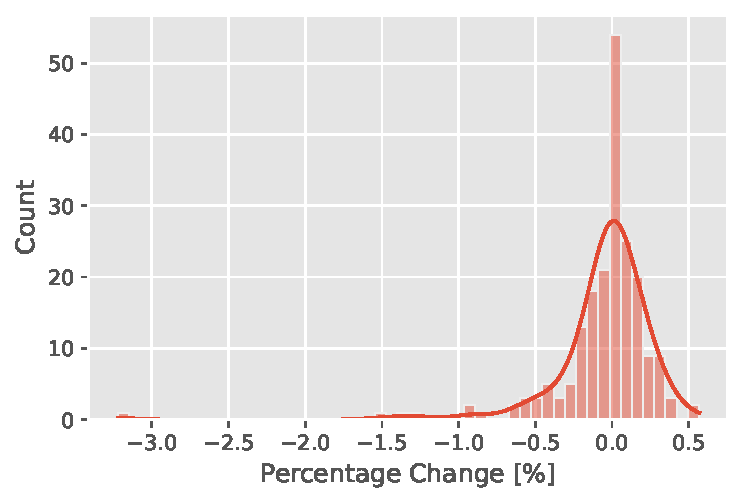
\includegraphics{compare_files/figure-pdf/fig-incl-compare-output-2.pdf}

}

\subcaption{\label{fig-incl-compare-2}Distribution of the Percentage
Change}

\end{minipage}%

\caption{\label{fig-incl-compare}Comparison of the Inclination of the
galaxies}

\end{figure}%

\begin{longtable}[]{@{}llll@{}}
\toprule\noalign{}
& inc & INCL & Percentage Change {[}\%{]} \\
\midrule\noalign{}
\endhead
\bottomrule\noalign{}
\endlastfoot
count & 1308 & 1994 & 202 \\
mean & 55 & 51 & -0 \\
std & 20 & 20 & 0 \\
min & 0 & 0 & -3 \\
50\% & 54 & 50 & 0 \\
max & 90 & 90 & 1 \\
\end{longtable}

We can see that for values in the range
\([\sim 30^\circ,\sim 80^\circ]\), the values of the LVG inclination are
higher (Figure~\ref{fig-incl-compare}). However, since their means,
median, min and maxes are similar and the percentage change is
practically 0\% (mean, median, \(\sigma\) = 0 with a range
\([-3\%,1\%]\)), we can ignore the differences and assume they are the
same values.

\subsubsection{Major Axis}

\begin{figure}

\begin{minipage}{0.50\linewidth}

\centering{

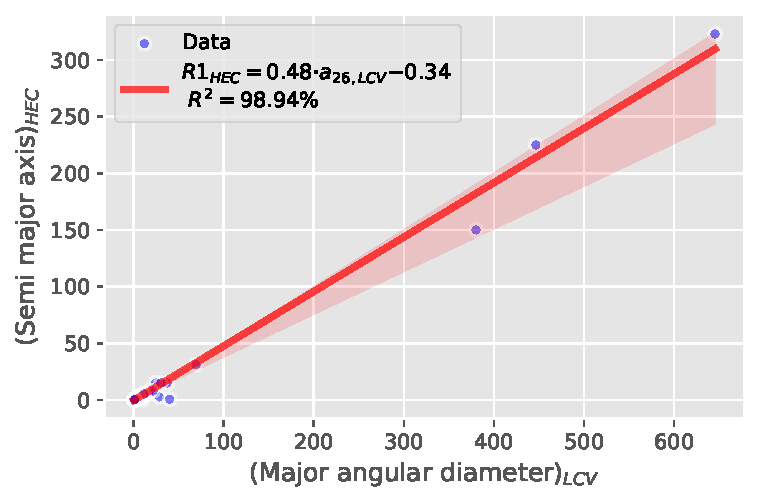
\includegraphics{compare_files/figure-pdf/fig-axis-compare-output-1.pdf}

}

\subcaption{\label{fig-axis-compare-1}Linear scale}

\end{minipage}%
%
\begin{minipage}{0.50\linewidth}

\centering{

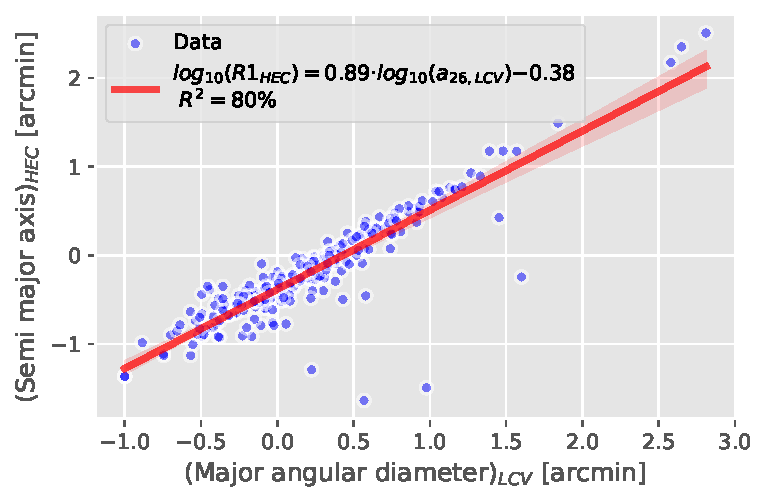
\includegraphics{compare_files/figure-pdf/fig-axis-compare-output-2.pdf}

}

\subcaption{\label{fig-axis-compare-2}\(log_{10}\) scale}

\end{minipage}%

\caption{\label{fig-axis-compare}Comparison of the Major Axises of the
galaxies}

\end{figure}%

it is not very clear if we truly have a correlation or not
(Figure~\ref{fig-axis-compare-1}). We need to see the linear correlation
of the decimal logarithms (Figure~\ref{fig-axis-compare-2}).

\(\overline{R_1} = 3.9\) {[}arcmin{]}, \(\overline{a_{26}} = 9.3\)
{[}arcmin{]}, so the intercept is negligable.

\[
R_1 = 0.48\cdot a_{26}-0.34 \sim \frac{1}{2}a_{26}
\]

\[
\log(R1) = 0.89\log(a_{26})-10^{0.38} = \log(10^{-0.38}a_{26}^{0.89}) = \log(0.41\cdot a_{26}^{0.89})\Rightarrow R1\simeq \frac{a_{26}}{2}
\]

\newpage{}

\subsection{Luminosities}\label{luminosities}

\begin{longtable}[]{@{}ccc@{}}
\toprule\noalign{}
LVG & HECATE & Description \\
\midrule\noalign{}
\endhead
\bottomrule\noalign{}
\endlastfoot
logKLum & logL\_K & \\
\end{longtable}

\begin{figure}

\begin{minipage}{0.50\linewidth}

\centering{

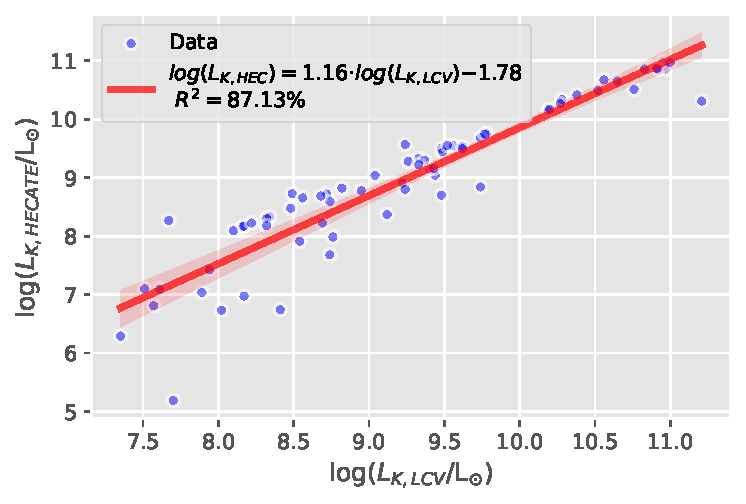
\includegraphics{compare_files/figure-pdf/fig-klum-compare-output-1.pdf}

}

\subcaption{\label{fig-klum-compare-1}Linear Regression with free
paramaters, \(y=ax+b\)}

\end{minipage}%
%
\begin{minipage}{0.50\linewidth}

\centering{

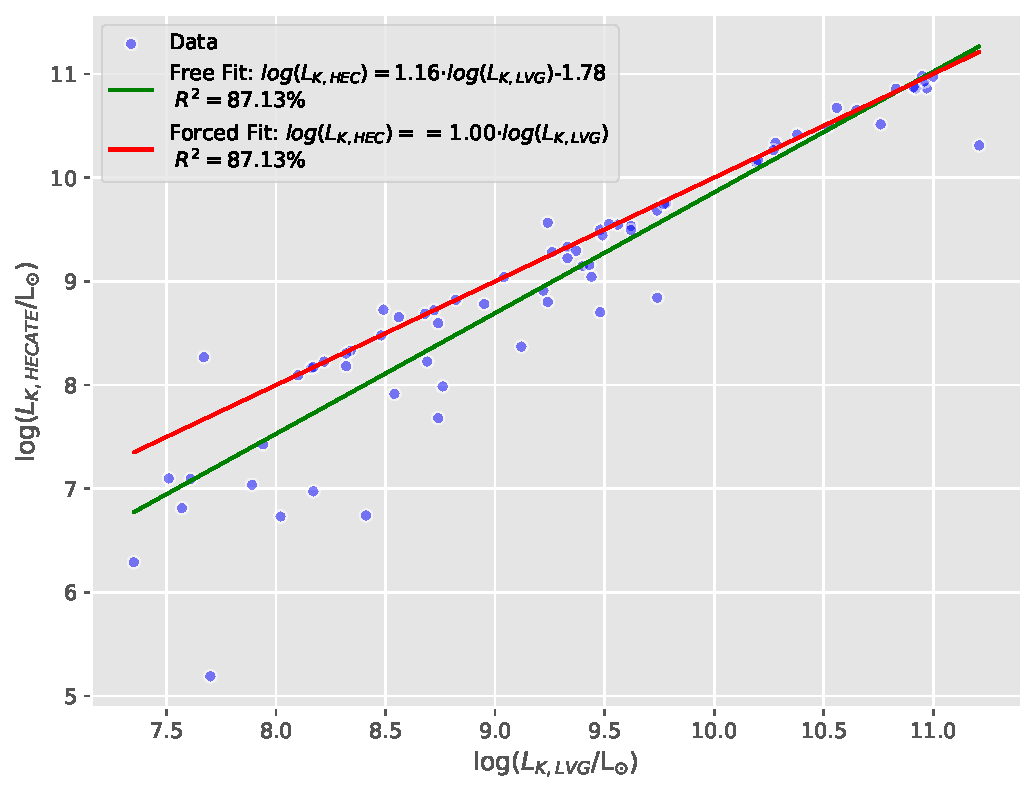
\includegraphics{compare_files/figure-pdf/fig-klum-compare-output-2.pdf}

}

\subcaption{\label{fig-klum-compare-2}Linear Regrassion \(y=x\)}

\end{minipage}%

\caption{\label{fig-klum-compare}Comparison of the \(L_K\) of the
galaxies.}

\end{figure}%

\[
\log(L_{K,HEC})=1.16\log(L_{K,LVG})-1.78=\log\left(\frac{{L_{K,LVG}}^{1.16}}{10^{1.78}}\right) \Leftrightarrow L_{K,HEC}=0.02\cdot{L_{K,LVG}}^{1.16}
\]

To assess whether the two galaxy catalogs have a 1-1 correlation, I
applied two types of linear fits to the data: a free fit and a forced
fit. The free fit allows both the slope and intercept to vary freely,
meaning the line can take on any slope and can cross the y-axis at any
point. In contrast, for the forced fit, I set the slope to exactly 1 and
fixed the line to pass through the origin, meaning the equation becomes
\(y=x\). This forced fit represents a perfect 1-1 relationship, where
the values from one catalog should match the other exactly, without any
shift or scaling.

After fitting the data using both methods, I calculated the \(R^2\)
value for each fit. In this case, both the free fit and the forced fit
produced very similar \(R^2\) values, around 87.13\%\footnote{The
  difference of the linear regression with the free parameters and the
  forced regression is \(\Delta R^2 = 1.14\cdot 10^{-13}\%\)},
indicating that both fits explain about 87\% of the variance in the data
(Figure~\ref{fig-klum-compare}).

The fact that both the free and forced fits have nearly identical
\(R^2\) values suggests that the data closely follows a 1-1
relationship. In the free fit, the best-fitting line had a very small
intercept, which shows that allowing the line to shift vertically did
not significantly improve how well the line fits the data. This strongly
indicates that the data from the two catalogs are well-aligned and
follow the relationship y=x quite closely, which is what we expect if
the catalogs are in good agreement.

While these results are promising, it's important to note that achieving
an \(R^2\) of 87\%---while high---doesn't necessarily prove a perfect
1-1 correlation. There may still be small discrepancies or uncertainties
in the data that prevent a perfect match. Nonetheless, the fact that
fixing the slope to 1 and forcing the line through the origin gave such
a good result suggests that the two catalogs are very consistent with
each other.

\subsection{Magnitudes}\label{magnitudes}

\begin{longtable}[]{@{}ccc@{}}
\toprule\noalign{}
LVG & HECATE & Description \\
\midrule\noalign{}
\endhead
\bottomrule\noalign{}
\endlastfoot
mag\_B (with errors) & BT (with errors) & \\
Kmag & K & 2MASS band magnitude (both) \\
\end{longtable}

\begin{figure}

\begin{minipage}{0.50\linewidth}

\centering{

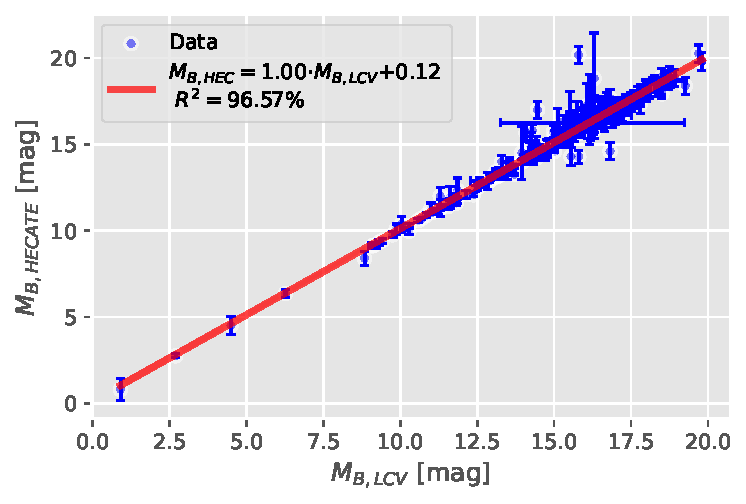
\includegraphics{compare_files/figure-pdf/fig-mag-compare-output-1.pdf}

}

\subcaption{\label{fig-mag-compare-1}\(M_B\)}

\end{minipage}%
%
\begin{minipage}{0.50\linewidth}

\centering{

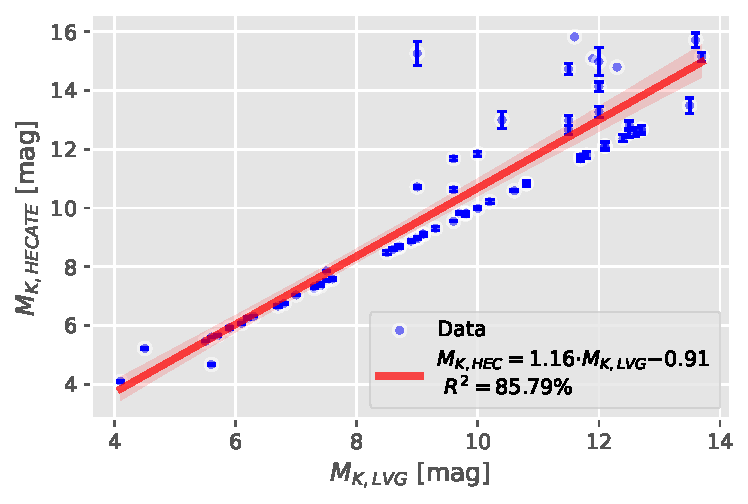
\includegraphics{compare_files/figure-pdf/fig-mag-compare-output-2.pdf}

}

\subcaption{\label{fig-mag-compare-2}\(M_K\)}

\end{minipage}%

\caption{\label{fig-mag-compare}Comparison of the Magnitudes of the
galaxies}

\end{figure}%

\begin{itemize}
\tightlist
\item
  \(M_B\): it is a 1-1 correlation, since the average error
  \(M_{B,HECATE} = 0.4\ mag\), so the itercept is smaller than the error
  (Figure~\ref{fig-mag-compare})
\item
  \(M_K\): we need to examine it more, since the intercept is bigger
  than the error \(M_{K,HECATE} = 0.09\ mag\)
  (Figure~\ref{fig-mag-compare})
\end{itemize}

\begin{figure}

\begin{minipage}{0.50\linewidth}

\centering{

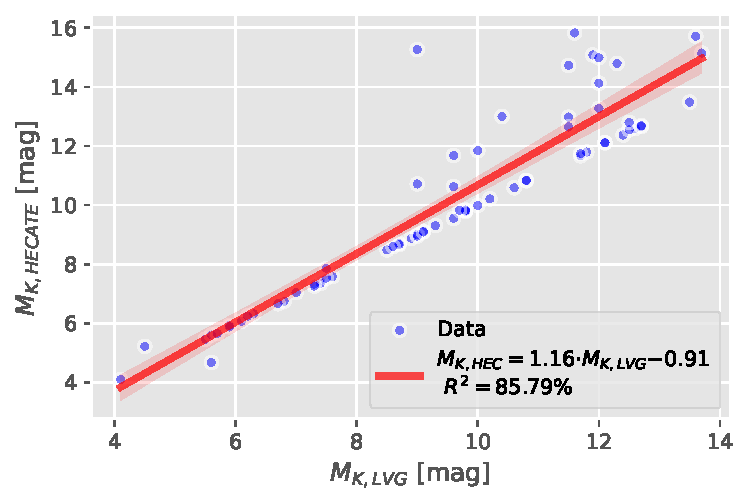
\includegraphics{compare_files/figure-pdf/fig-kmag-compare-output-1.pdf}

}

\subcaption{\label{fig-kmag-compare-1}Linear Regression with free
paramaters, \(y=ax+b\)}

\end{minipage}%
%
\begin{minipage}{0.50\linewidth}

\centering{

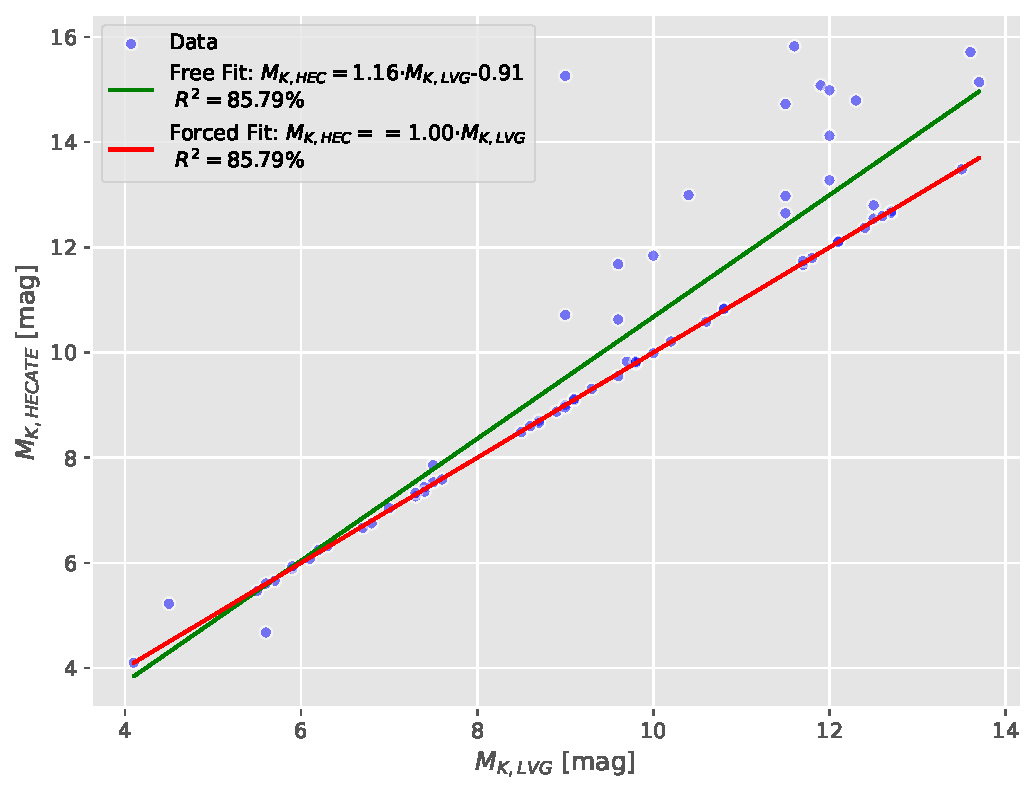
\includegraphics{compare_files/figure-pdf/fig-kmag-compare-output-2.pdf}

}

\subcaption{\label{fig-kmag-compare-2}Linear Regrassion \(y=x\)}

\end{minipage}%

\caption{\label{fig-kmag-compare}Comparison of the \(L_K\) of the
galaxies.}

\end{figure}%

Following the same logic as in Figure~\ref{fig-klum-compare}, we force
the parameters of the linear regression to be \(y=1\cdot x + 0\).

In this case, the data is such that both the forced fit and the free fit
explain the variance almost identically
(Figure~\ref{fig-kmag-compare-2}). This can happen when the data roughly
follows the pattern \(y≈x\), but with a slight bias that the free fit
can account for (in this case, a slope slightly greater than 1 and a
negative intercept).

\newpage{}

\subsection{SFR}\label{sfr}

\begin{longtable}[]{@{}
  >{\centering\arraybackslash}p{(\columnwidth - 4\tabcolsep) * \real{0.3273}}
  >{\centering\arraybackslash}p{(\columnwidth - 4\tabcolsep) * \real{0.3273}}
  >{\centering\arraybackslash}p{(\columnwidth - 4\tabcolsep) * \real{0.3455}}@{}}
\toprule\noalign{}
\begin{minipage}[b]{\linewidth}\centering
LVG
\end{minipage} & \begin{minipage}[b]{\linewidth}\centering
HECATE
\end{minipage} & \begin{minipage}[b]{\linewidth}\centering
Description
\end{minipage} \\
\midrule\noalign{}
\endhead
\bottomrule\noalign{}
\endlastfoot
& logSFR\_TIR & Decimal logarithm of the total-infrared SFR estimate
{[}Msol/yr{]} \\
& logSFR\_FIR & Decimal logarithm of the far-infrared SFR estimate
{[}Msol/yr{]} \\
& logSFR\_60u & Decimal logarithm of the 60um SFR estimate
{[}Msol/yr{]} \\
& logSFR\_12u & Decimal logarithm of the 12um SFR estimate
{[}Msol/yr{]} \\
& logSFR\_22u & Decimal logarithm of the 22um SFR estimate
{[}Msol/yr{]} \\
& logSFR\_HEC & Decimal logarithm of the homogenised SFR estimate
{[}Msol/yr{]} \\
& logSFR\_GSW & Decimal logarithm of the SFR in GSWLC-2 {[}Msol/yr{]} \\
SFRFUV & & FUV derived integral star formation rate \\
SFRHa & & H\{alpha\} derived integral star formation rate \\
\end{longtable}

\begin{figure}

\centering{

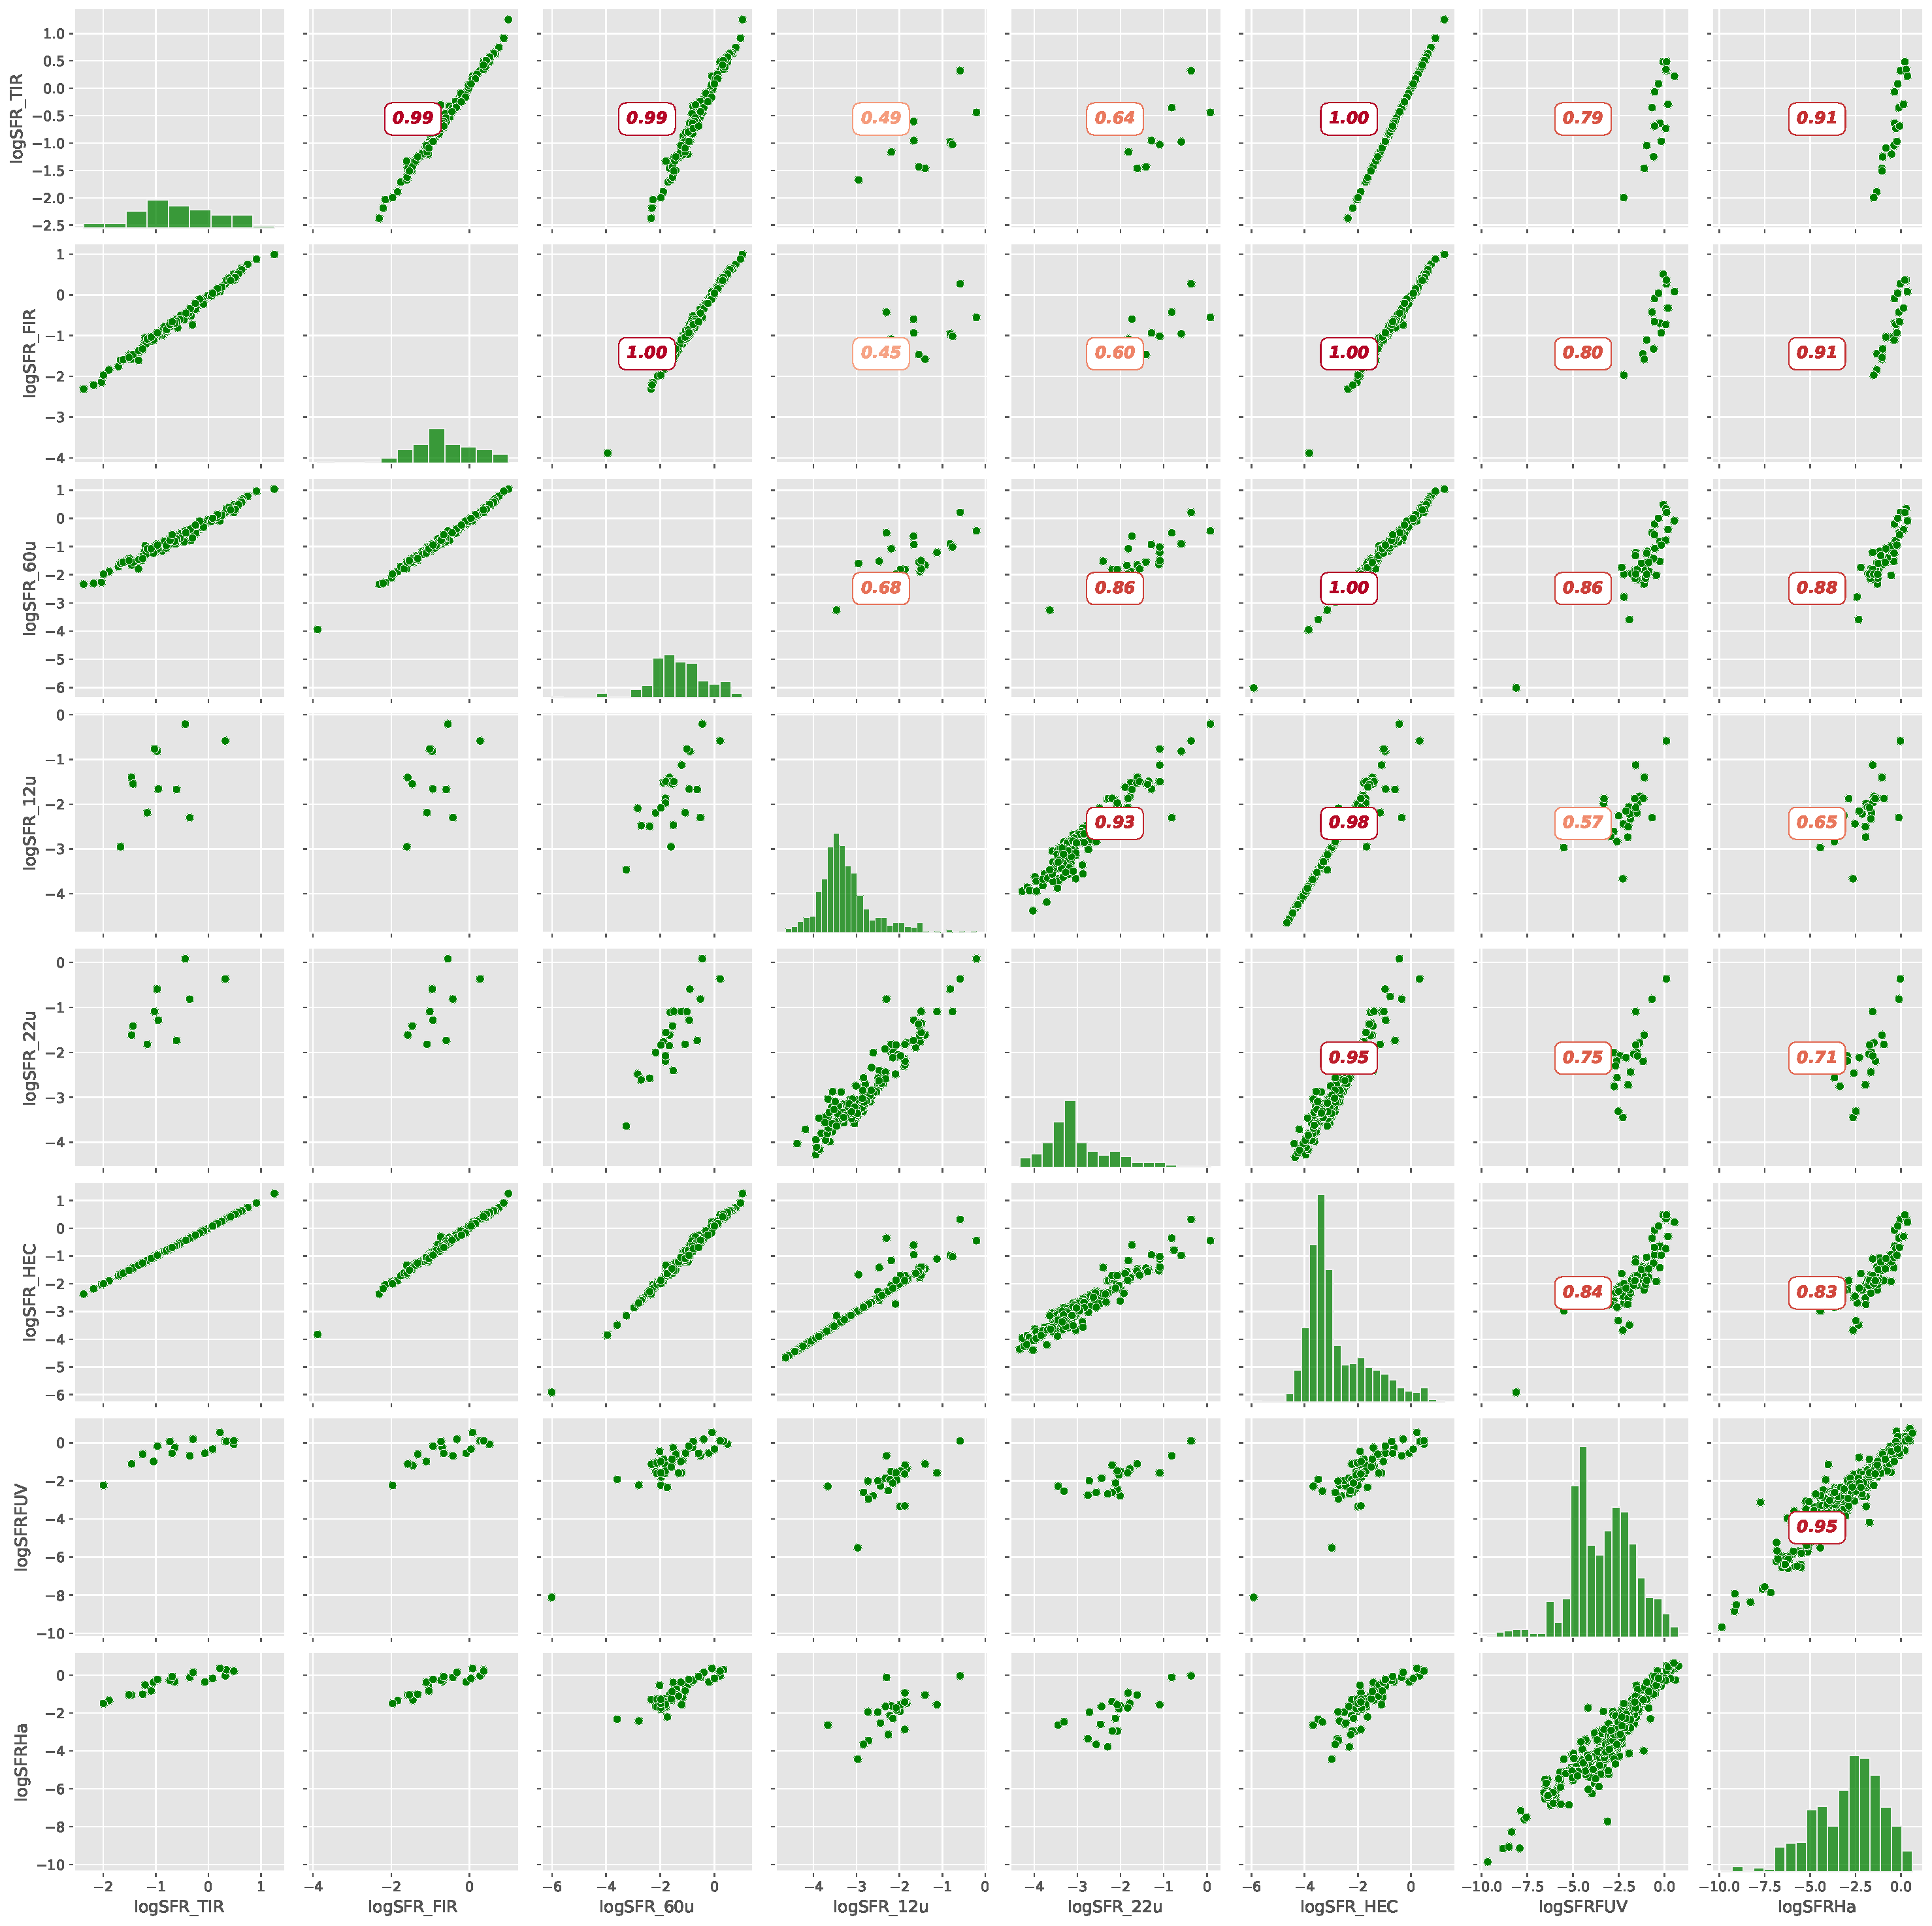
\includegraphics{compare_files/figure-pdf/fig-sfr-pairplot-output-1.pdf}

}

\caption{\label{fig-sfr-pairplot}Comparison of the \(SFR_{i}\) of the
galaxies}

\end{figure}%

The SFR according to (Kroupa et al. (2020)), can be calculated from the
mean of SFR from the Ha and FUV, for \(SFR>10^{-3}\ M_\odot\, yr^{-1}\).
As we can see from the plots (Figure~\ref{fig-sfr-lvg}) it could be a
good aproximation.

\begin{equation}\phantomsection\label{eq-sfr-mean}{
SFR = \frac{SFR_{FUV}+SFR_{H\alpha}}{2}, \text{if both exist, else: } SFR = SFR_i,\ i= FUV,\, H\alpha
}\end{equation}

\begin{figure}

\begin{minipage}{0.50\linewidth}

\centering{

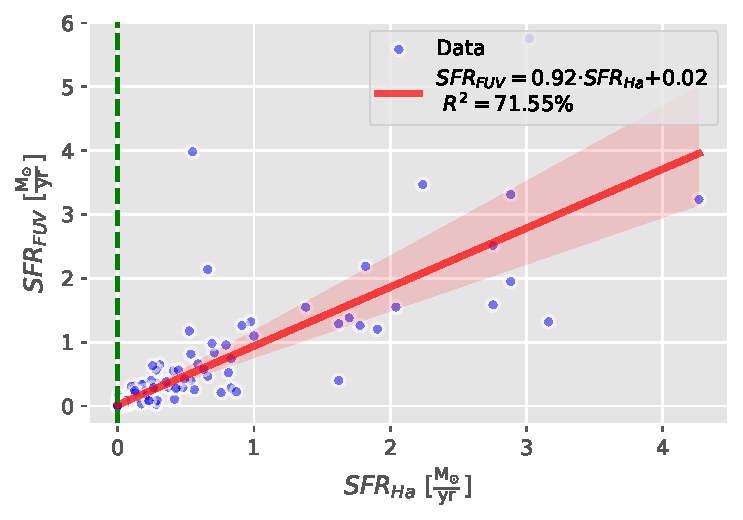
\includegraphics{compare_files/figure-pdf/fig-sfr-lvg-output-1.pdf}

}

\subcaption{\label{fig-sfr-lvg-1}Linear scale}

\end{minipage}%
%
\begin{minipage}{0.50\linewidth}

\centering{

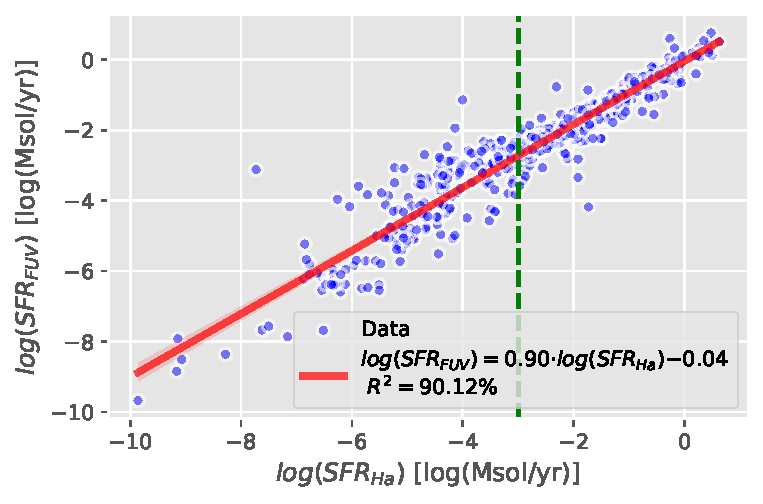
\includegraphics{compare_files/figure-pdf/fig-sfr-lvg-output-2.pdf}

}

\subcaption{\label{fig-sfr-lvg-2}Decimal logarithmic scale}

\end{minipage}%

\caption{\label{fig-sfr-lvg}Comparison of the \(SFR_{FUV}-SFR_{Ha}\) of
the galaxies}

\end{figure}%

\begin{figure}

\begin{minipage}{0.50\linewidth}

\centering{

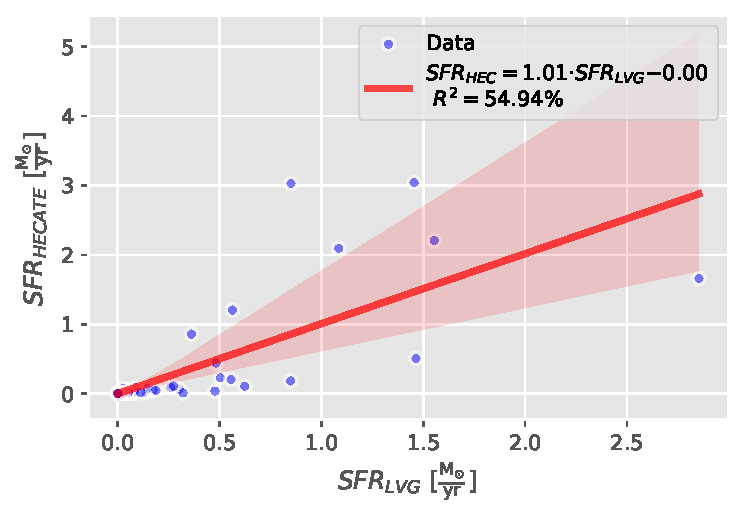
\includegraphics{compare_files/figure-pdf/fig-sfr-compare-output-1.pdf}

}

\subcaption{\label{fig-sfr-compare-1}Linear scale}

\end{minipage}%
%
\begin{minipage}{0.50\linewidth}

\centering{

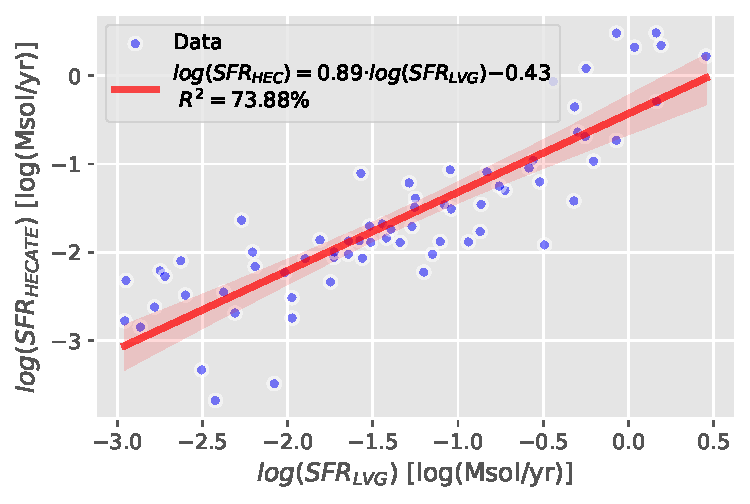
\includegraphics{compare_files/figure-pdf/fig-sfr-compare-output-2.pdf}

}

\subcaption{\label{fig-sfr-compare-2}Decimal logarithmic scale}

\end{minipage}%

\caption{\label{fig-sfr-compare}Comparison of the SFR's of the galaxies}

\end{figure}%

The low correlation in Figure~\ref{fig-sfr-compare-1} and the interval
in Figure~\ref{fig-sfr-compare-2} show that the approximation
(Equation~\ref{eq-sfr-mean}) is not great. According to Karachentsev and
Kaisina (2013):

\begin{itemize}
\item
  \textbf{Hα and FUV timescales}: \(H_\alpha\) traces short-term star
  formation (\textasciitilde10 Myr) via massive O-type stars, while FUV
  traces longer-term star formation (\textasciitilde100 Myr) from B-type
  stars.
\item
  \textbf{Discrepancies due to star formation bursts}: In galaxies with
  bursty or episodic star formation, Hα can significantly overestimate
  SFR compared to FUV, which lags in reflecting recent star formation
  events.
\item
  \textbf{Low-mass galaxy variability}: The scatter between
  \(SFR_{\text{H}\alpha}\) and \(SFR_{\text{FUV}}\) is particularly high
  in low-mass, dwarf galaxies, where stochastic star formation history
  causes wide variability between the two indicators.
\item
  \textbf{Measurement uncertainties}: Internal extinction, errors in
  distance estimates, and IMF stochasticity introduce biases in both Hα
  and FUV fluxes, making simple averaging inappropriate.
\item
  \textbf{Conclusion}: The
  \(SFR_{\text{total}} = \text{mean}(SFR_{\text{H}\alpha}, SFR_{\text{FUV}})\)
  method oversimplifies the complexity of star formation processes and
  is not reliable for galaxies with variable star formation or
  significant measurement uncertainties
\end{itemize}

\newpage{}

\subsection{Masses}\label{masses}

\begin{longtable}[]{@{}
  >{\centering\arraybackslash}p{(\columnwidth - 4\tabcolsep) * \real{0.3333}}
  >{\centering\arraybackslash}p{(\columnwidth - 4\tabcolsep) * \real{0.3333}}
  >{\centering\arraybackslash}p{(\columnwidth - 4\tabcolsep) * \real{0.3333}}@{}}
\toprule\noalign{}
\begin{minipage}[b]{\linewidth}\centering
LVG
\end{minipage} & \begin{minipage}[b]{\linewidth}\centering
HECATE
\end{minipage} & \begin{minipage}[b]{\linewidth}\centering
Description
\end{minipage} \\
\midrule\noalign{}
\endhead
\bottomrule\noalign{}
\endlastfoot
logM26 & & Log mass within Holmberg radius \\
logMHI & & Log mass within Holmberg radius \\
& logM\_HEC & Decimal logarithm of the stellar mass {[}Msol{]} \\
& logM\_GSW & Decimal logarithm of the stellar mass in GSWLC-2
{[}Msol{]} \\
logStellarMass & & Stellar Mass from \(M_*/L=0.6\) \\
\end{longtable}

\subsubsection{Stellar Masses Comparison}

\newpage{}

\begin{figure}

\centering{

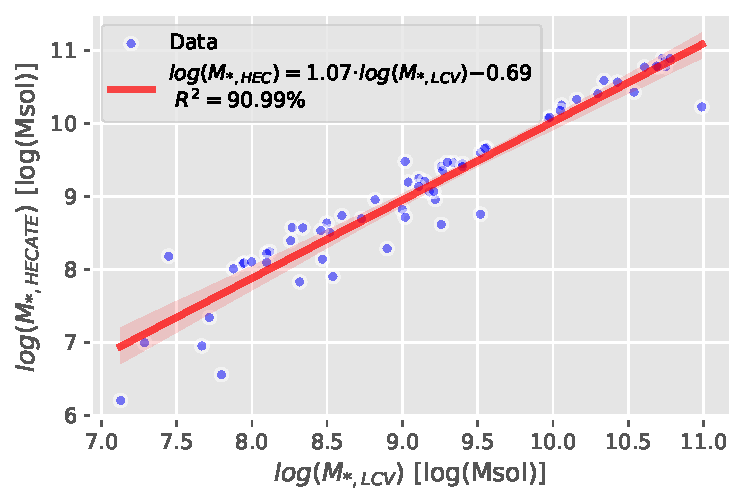
\includegraphics{compare_files/figure-pdf/fig-mass-compare-output-1.pdf}

}

\caption{\label{fig-mass-compare}Comparison of the Stellar Masses of the
galaxies}

\end{figure}%

\[
\log{M_{*,HECATE}}=1.07\cdot\log{M_{*,LVG}}-0.69, \text{ but } \log{M_*}>6\Rightarrow M_{*,HEC}\sim M_{*,LVG}
\]

As we can see the aproximation of Mass/Light=const.=0.6 is a pretty good
approximation, for the calculation of \(\log(M_*/M_\odot)\), especially
for high-mass galaxies

\newpage{}

\subsubsection{Heatmap}

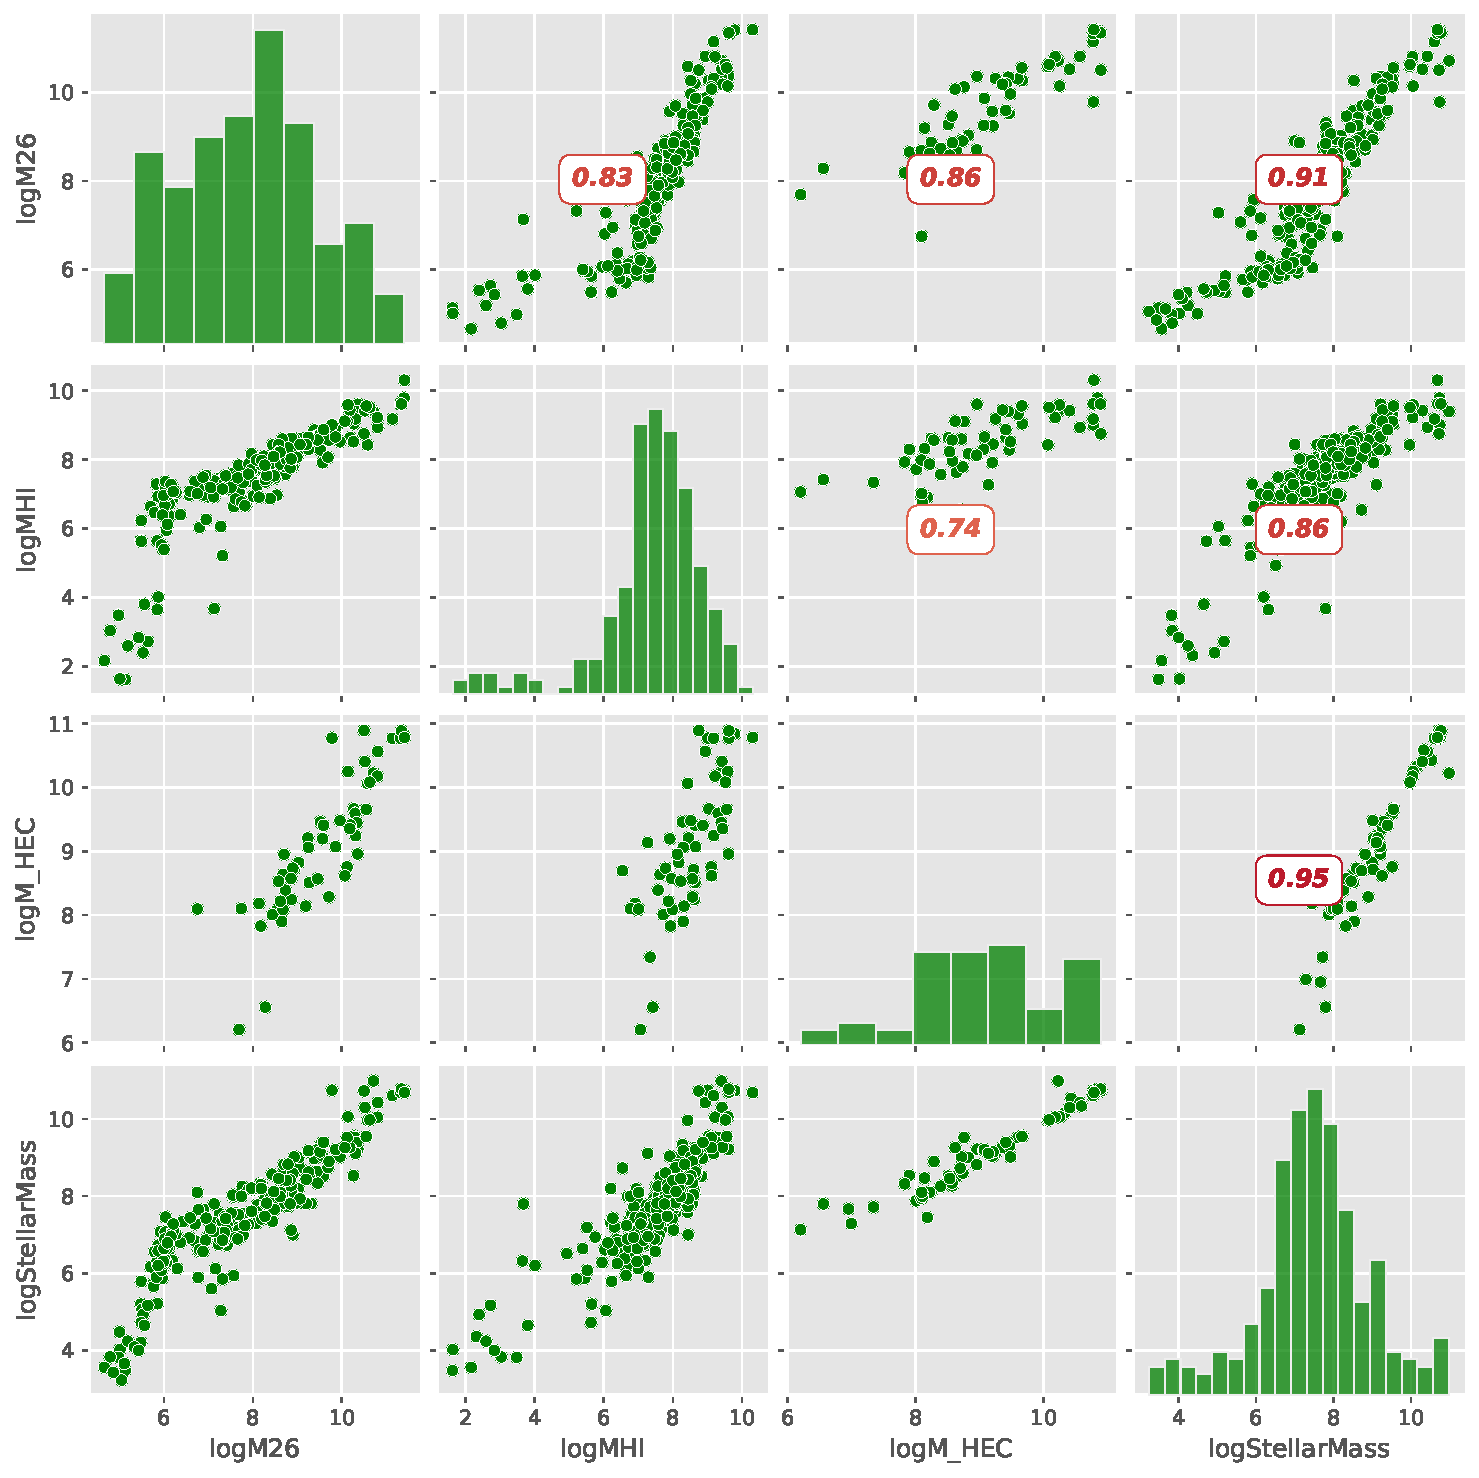
\includegraphics{compare_files/figure-pdf/cell-31-output-1.pdf}

The heatmap is used to visually assess the correlations between
different mass estimates of the galaxies, including the mass within the
Holmberg radius (\(M_{26}\)), the HI gas mass (\(M_{HI}\)\hspace{0pt}),
the stellar mass from the HECATE catalog (\(M_{HEC}\)\hspace{0pt}), and
the stellar mass derived assuming a mass-to-light ratio of 0.6
(StellarMass). The purpose of this visualization is to quickly identify
whether these different mass measurements show consistent correlations,
which would suggest that they capture similar aspects of the galaxies'
mass distributions.

This quick check using the heatmap helps confirm that, while different
catalogs and methods might have their own specific ways of calculating
galaxy masses, the overall mass estimates align well, offering a solid
basis for further analysis of galaxy properties.

\begin{center}\rule{0.5\linewidth}{0.5pt}\end{center}

\phantomsection\label{refs}
\begin{CSLReferences}{1}{0}
\bibitem[\citeproctext]{ref-Essay}
{``Essay.''} n.d. Accessed October 5, 2024.
\url{https://ned.ipac.caltech.edu/level5/Glossary/Essay_pecmotion.html}.

\bibitem[\citeproctext]{ref-karachentsevSTARFORMATIONPROPERTIES2013a}
Karachentsev, Igor D., and Elena I. Kaisina. 2013. {``{STAR FORMATION
PROPERTIES IN THE LOCAL VOLUME GALAXIES VIA Hα AND FAR-ULTRAVIOLET
FLUXES}.''} \emph{The Astronomical Journal} 146 (3): 46.
\url{https://doi.org/10.1088/0004-6256/146/3/46}.

\bibitem[\citeproctext]{ref-karachentsevUPDATEDNEARBYGALAXY2013}
Karachentsev, Igor D., Dmitry I. Makarov, and Elena I. Kaisina. 2013.
{``{UPDATED NEARBY GALAXY CATALOG}.''} \emph{The Astronomical Journal}
145 (4): 101. \url{https://doi.org/10.1088/0004-6256/145/4/101}.

\bibitem[\citeproctext]{ref-kovlakasHeraklionExtragalacticCatalogue2021}
Kovlakas, K., A. Zezas, J. J. Andrews, A. Basu-Zych, T. Fragos, A.
Hornschemeier, K. Kouroumpatzakis, B. Lehmer, and A. Ptak. 2021. {``The
{Heraklion Extragalactic Catalogue} ({HECATE}): A Value-Added Galaxy
Catalogue for Multimessenger Astrophysics.''} \emph{Monthly Notices of
the Royal Astronomical Society} 506 (September): 1896--1915.
\url{https://doi.org/10.1093/mnras/stab1799}.

\bibitem[\citeproctext]{ref-kroupaConstraintsStarFormation2020}
Kroupa, P, M Haslbauer, I Banik, S T Nagesh, and J Pflamm-Altenburg.
2020. {``Constraints on the Star Formation Histories of Galaxies in the
{Local Cosmological Volume}.''} \emph{Monthly Notices of the Royal
Astronomical Society} 497 (1): 37--43.
\url{https://doi.org/10.1093/mnras/staa1851}.

\bibitem[\citeproctext]{ref-navarroStructureColdDark1996}
Navarro, Julio F., Carlos S. Frenk, and Simon D. M. White. 1996. {``The
{Structure} of {Cold Dark Matter Halos}.''} \emph{The Astrophysical
Journal} 462 (May): 563. \url{https://doi.org/10.1086/177173}.

\end{CSLReferences}



\end{document}
